%%% Copyright (C) 2017 Vincent Goulet
%%%
%%% Ce fichier fait partie du projet «Programmer avec R»
%%% http://github.com/vigou3/programmer-avec-r
%%%
%%% Cette création est mise à disposition selon le contrat
%%% Attribution-Partage dans les mêmes conditions 4.0
%%% International de Creative Commons.
%%% http://creativecommons.org/licenses/by-sa/4.0/

\chapter{Travail collaboratif}
\label{chap:collaboration}

\begin{objectifs}
\item Employer les normes de programmation reconnues en matière de
  segmentation du code, de style et de documentation.
\item Créer une version locale d'un projet informatique hébergé dans
  un dépôt utilisant le système de gestion de version Git.
\item Créer, utiliser et supprimer une branche dans un projet avec
  Git.
\item Publier des ajouts et des modifications à un projet avec Git.
\item Rendre disponibles des ajouts et des modifications à une
  communauté par le biais d'un serveur Git.
\end{objectifs}

De manière générale, le développement et la maintenance de code
informatique repose sur la contribution de plusieurs personnes. En
effet, il est plutôt rare, dans le milieu professionnel, d'être appelé
à concevoir un programme informatique à partir d'une page blanche et
en complète autarcie, c'est-à-dire sans que quiconque n'ait à
interagir avec le code à un stade ou à un autre. Une grande part du
travail de programmation consiste à corriger, à mettre à jour ou à
améliorer du code existant. Dans ce contexte, l'adhésion à un certain
nombre de normes et de bonnes pratiques permet de faciliter le travail
de tous les intervenants et de réduire les risques d'erreurs. Ce
chapitre présente quelques unes de ces bonnes pratiques à adopter en
matière de style de programmation, de présentation du code et de
documentation.

Autre élément fondamental lors de travail collaboratif: le partage et
l'échange des contributions de chacun. Comment rendre le travail de
Marianne disponible à Alexandre? Comment s'assurer qu'une modification
apportée dans un fichier par Alexandre n'écrase pas celle sur laquelle
Marianne travaille depuis plusieurs heures? Comment identifier à coup
sûr et automatiquement la plus récente version d'un fichier? Ce genre
de questions, auxquelles quiconque a déjà travaillé en équipe sur un
projet a déjà été confronté, les informaticiens y ont répondu depuis
de très nombreuses années avec les systèmes de gestion de versions.
J'offre, dans ce chapitre, une courte introduction à ces outils de
développement incontournables avant de vous diriger vers la
documentation officielle du système de gestion le plus utilisé dans le
monde en ce moment: Git.


\section{Style}
\label{sec:collaboration:style}

Il en va du code informatique comme de la prose: si le style peut
varier d'un auteur à l'autre, l'œuvre doit toujours être à la fois
agréable à lire et facile à comprendre. Bref, les meilleurs
programmeurs préfèrent la \emph{lisibilité} de leur code aux effets de
style qui n'auraient pour seul mérite d'afficher leur maitrise du
langage.

Tout programmeur devrait constamment garder en tête les trois
objectifs suivants en effectuant son travail: simplicité, clarté,
concision. Ces objectifs entrent souvent en conflit les uns avec les
autres! Tout l'art de la bonne programmation consiste donc à trouver
un juste équilibre entre les trois pôles.

\citet{Kernighan:practice:1999},
\citet{Oualline:C:1997,Oualline:C++:2003},
\citet{Kernighan:style:1978} proposent d'excellents chapitres sur le
style en programmation. Je ne saurais être aussi exhaustif que ces
auteurs établis. Néanmoins, je vous incite à porter une attention
particulière aux quelques points de style livrés en vrac, ci-dessous.

\begin{itemize}
\item Utilisez des noms de variables significatifs. Ne soyez pas ce
  collègue qui nomme les variables d'un programme \code{x}, \code{xx}
  et \code{xxx} (cas vécu). Attention, toutefois, de ne pas pousser le
  concept trop loin. Ici comme ailleurs, la clarté peut provenir de la
  concision; la terminologie\footnote{%
    Vous remarquerez que je préfère utiliser l'anglais pour les
    noms d'objets, question d'uniformité avec les identificateurs du
    langage. Chose certaine, évitez à tout prix les accents dans les
    noms d'objets.}
  \begin{Schunk}
\begin{Verbatim}
xlen <- length(x)
\end{Verbatim}
  \end{Schunk}
  est aussi claire que
  \begin{Schunk}
\begin{Verbatim}
length_of_x <- length(x)
\end{Verbatim}
  \end{Schunk}
  et bien plus simple à utiliser au fil d'un programme.

  Certains noms d'objets sans réelle signification sont tellement
  usuels qu'il est contre productif de leur préférer des versions plus
  explicites. Pensons, ici, à \code{x} comme premier argument d'une
  fonction R ou à \code{i}, \code{j} et \code{k} comme compteurs dans
  les boucles \icode{for}.

  Quant à la composition des noms d'objets formés de plusieurs mots,
  divers styles s'affrontent: \code{variable.name},
  \code{variable\_name}, \code{variableName}, \code{VariableName},
  etc. Assurez-vous simplement de suivre le standard en vigueur dans
  votre équipe de travail, le cas échéant, et, par-dessus tout, soyez
  constant. Notre préférence, qui concorde avec une grande partie du
  code source de R, va aux noms d'objets courts et entièrement en
  minuscules.
  %
\item Dès qu'elles sont disponibles, utilisez les fonctions internes
  de R au lieu de reprogrammer certaines procédures. Non seulement
  bénéficierez-vous de l'optimisation des fonctions internes, mais
  votre code gagnera également en lisibilité. Comparez
  \begin{Schunk}
\begin{Verbatim}
sum(x)/length(x)
\end{Verbatim}
  \end{Schunk}
  à
  \begin{Schunk}
\begin{Verbatim}
mean(x)
\end{Verbatim}
  \end{Schunk}
  %
\item Connaitre sur le bout des doigts la priorité des opérateurs du
  \autoref{tab:bases:operateurs}, c'est bien; rendre explicite l'ordre
  des opérations dans une expression à l'aide de parenthèses, c'est
  mieux. N'hésitez pas à utiliser des parenthèses dès que l'ombre d'un
  doute pourrait planer sur l'ordre des opérations. D'ailleurs, à ce
  propos, \citet{Oualline:C:1997} ramène la quinzaine de règles de
  priorité des opérations (du langage C) à seulement deux:
  \begin{enumerate}
  \item La multiplication et la division précèdent l'addition et la
    soustraction.
  \item Placer tout le reste entre parenthèses.
  \end{enumerate}
  %
\item Évitez les expressions logiques complexes, surtout celles
  reposant sur la double négation. Par exemple, pour exécuter une
  expression si un vecteur contient des données manquantes, la
  condition
  \begin{Schunk}
\begin{Verbatim}
if (any(is.na(x)))
\end{Verbatim}
  \end{Schunk}
  est beaucoup plus facile à déchiffrer que la version équivalente
  d'un point de vue logique
  \begin{Schunk}
\begin{Verbatim}
if (!all(!is.na(x)))
\end{Verbatim}
  \end{Schunk}
  En revanche, s'il s'agit plutôt d'exécuter une expression quand un
  vecteur ne contient aucune donnée manquante, alors
  \begin{Schunk}
\begin{Verbatim}
if (all(!is.na(x)))
\end{Verbatim}
  \end{Schunk}
  est plus simple que
  \begin{Schunk}
\begin{Verbatim}
if (!any(is.na(x)))
\end{Verbatim}
  \end{Schunk}

  De plus, le conseil précédent sur la priorité des opérations est
  particulièrement indiqué avec les opérations logiques. Sauriez-vous
  confirmer, sans consulter le \autoref{tab:bases:operateurs}, l'ordre
  des opérations dans l'expression logique suivante?\footnote{%
    C'est \code{(!p) | (q \& r)}.}
  \begin{Schunk}
\begin{Verbatim}
!p | q & r
\end{Verbatim}
  \end{Schunk}
  %
\item Utilisez les fonctions d'application
  (\autoref{chap:application}) plutôt que des boucles explicites. Une
  expression ayant recours à une fonction d'application est plus
  concise et plus simple à décoder. Comparez
  \begin{Schunk}
\begin{Verbatim}
z <- numeric(n)
for (i in seq_len(n))
    z[i] <- mean(x[[i]])
\end{Verbatim}
  \end{Schunk}
  et
  \begin{Schunk}
\begin{Verbatim}
z <- sapply(x, mean)
\end{Verbatim}
  \end{Schunk}

  Encore ici, évitez de pousser la logique trop loin. Si une boucle
  est plus naturelle et plus simple à comprendre qu'une fonction
  d'application, optez pour la boucle. En particulier, une
  fonction d'application \icode{sapply} à l'intérieur d'une autre
  fonction \code{sapply}, ce n'est généralement ni plus efficace, ni
  plus simple à déchiffrer qu'une double boucle \icode{for}.
  %
\item Adoptez la
  \link{https://fr.wikipedia.org/wiki/Philosophie_d\%27Unix}{philosophie
    Unix}, notamment le précepte qui appelle à créer des programmes
  qui effectuent une seule chose et qui le font bien. Lorsqu'une
  fonction devient «longue» --- cela dépend du contexte, mais
  généralement dès une vingtaine de lignes en R --- il convient de la
  scinder en plusieurs blocs logiques.
  %
\item Enfin, utilisez \icode{return} uniquement pour provoquer la
  sortie anticipée d'une fonction, habituellement à l'intérieur d'une
  clause \code{if}. En d'autres termes, \code{return} n'a pas sa
  place, en R, à la toute fin d'une fonction.
\end{itemize}


\section{Présentation du code}
\label{sec:collaboration:presentation}

Le code bien mis en forme est plus facile et agréable à consulter. Il
existe plusieurs chapelles dans le monde des programmeurs quant à la
«bonne façon» de présenter et, surtout, d'indenter le code
informatique.

Voyons d'abord ce qui rallie tout le monde.

En premier lieu, veillez à limiter la longueur des lignes de code à
environ 80 caractères. Ce standard remonte à l'époque des terminaux en
format texte qui ne pouvaient afficher de l'information que sur 80
colonnes. Pourquoi s'y tenir encore aujourd'hui, alors que nos écrans
d'ordinateur sont très larges? Parce que les longues lignes de texte
sont difficile à suivre, notre œil ayant tendance à sauter à la ligne
inférieure en se déplaçant de la gauche vers la droite\footnote{%
  C'est pourquoi les journaux et les magazines sont composés en
  colonnes de texte étroites.}. %
Profitez donc plutôt de l'espace horizontal à l'écran pour afficher
des fenêtres côte-à-côte.

Si de multiples niveaux d'indentation (voir plus bas) font en sorte
qu'il manque de place à droite pour écrire du code, le problème n'est
peut-être pas tant la limite sur la longueur des lignes que la
conception même du programme. Simplifiez l'algorithme ou scindez le
programme en plusieurs fonctions.

Ensuite, aérez le code avec des lignes blanches entre les blocs
logiques et, surtout, avec des espaces. Les espaces en programmation
jouent le même rôle que dans du texte normal: elles facilitent la
lecture. En particulier, utilisez des espaces dans les circonstances
suivantes:
\begin{itemize}
\item de part et d'autre du symbole d'affectation \icode{<-}; ces
  espaces sont ajoutées automatiquement avec les raccourcis clavier
  des éditeurs spécialisés GNU~Emacs
  (\autoref{sec:emacs+ess:commandes:script}) et RStudio
  (\autoref{sec:rstudio:commandes});
\item de part et d'autre de tous les opérateurs\footnote{%
    Sauf peut-être la division: je préfère \code{(x + y)/z} à \code{(x
      + y) / z}.};
\item après les virgules;
\item avant la parenthèse ouvrante \code{(}, sauf dans les appels de
  fonction.
\end{itemize}
Comparez les deux blocs de code de la
\autoref{fig:collaboration:espaces}. Vous serez sans doute d'accord
que celui qui respecte les indications ci-dessus s'avère bien plus
lisible.

\begin{figure}
  \begin{minipage}{0.48\linewidth}
    \begin{Schunk}
\begin{Verbatim}
f<-function(x,y)
{
    if(y<0)
        y<--y
    x*(1+x*y)^2
}
\end{Verbatim}
    \end{Schunk}
  \end{minipage}
  \hfill
  \begin{minipage}{0.48\linewidth}
    \begin{Schunk}
\begin{Verbatim}
f <- function(x, y)
{
    if (y < 0)
        y <- -y
    x * (1 + x * y)^2
}
\end{Verbatim}
    \end{Schunk}
  \end{minipage}
  \caption{Blocs de code sans (à gauche) et avec (à droite) les
    espaces appropriées. Le code de droite est plus lisible.}
  \label{fig:collaboration:espaces}
\end{figure}

Passons maintenant au dossier chaud parmi les programmeurs:
l'indentation du code et la position des accolades. Tous s'entendent
au moins sur un point: il est absolument essentiel d'indenter les
blocs de code pour mettre la structure d'un programme en évidence. En
clair, cela signifie que toute expression --- ou groupe d'expressions
entre accolades --- doit être placé en retrait de la marge de gauche
dès lors qu'elle fait partie d'une structure de contrôle ou de la
définition d'une fonction. Le code de la
\autoref{fig:collaboration:espaces} est correctement indenté.

\importantbox{Ne pas du tout indenter son code est passible de la
  peine capitale, d'excommunication, de bannissement de la Terre du
  Milieu\dots\ choisissez votre châtiment.}

La source des insolubles débats se situe, comme souvent, dans les
détails: le nombre d'espaces dont il convient d'indenter le code et la
position des accolades, surtout l'accolade ouvrante. À titre
d'exemples, l'éditeur GNU~Emacs\index{Emacs} reconnaît et supporte au
moins les styles d'indentation suivants:

\vspace{\topsep}\noindent
\begin{minipage}{\linewidth}
  \begin{minipage}[t]{0.48\linewidth}
    C++
    \begin{Schunk}
\begin{Verbatim}
for (i in 1:10)
{
    expression
}
\end{Verbatim}
    \end{Schunk}
  \end{minipage}
  \hfill
  \begin{minipage}[t]{0.48\linewidth}
    K\&R (1TBS\footnotemark)
    \begin{Schunk}
\begin{Verbatim}
for (i in 1:10){
     expression
}
\end{Verbatim}
    \end{Schunk}
  \end{minipage}
\end{minipage}
\footnotetext{\emph{One True Bracing Style}. C'est dire
  combien les amateurs de ce style le tiennent en haute estime.}

\vspace{\topsep}\noindent
\begin{minipage}{\linewidth}
  \begin{minipage}[t]{0.48\linewidth}
    Whitesmith
    \begin{Schunk}
\begin{Verbatim}
for (i in 1:10)
     {
     expression
     }
\end{Verbatim}
    \end{Schunk}
  \end{minipage}
  \hfill
  \begin{minipage}[t]{0.48\linewidth}
    GNU
    \begin{Schunk}
\begin{Verbatim}
for (i in 1:10)
  {
    expression
  }
\end{Verbatim}
    \end{Schunk}
  \end{minipage}
\end{minipage}
\vspace{\topsep}

Le code source de R est entièrement composé dans un style analogue aux
style C++, ci-dessus, ou RRR du \index{Emacs!mode ESS}mode ESS de Emacs:
\begin{itemize}
\item le code est indenté de quatre (4) espaces;
\item les accolades ouvrante et fermante sont placées sur leurs
  propres lignes.
\end{itemize}
Ce style peut être  considéré comme standard pour la programmation en
R.

En définitive, le style d'indentation utilisé n'a pas tellement
d'importance. Ce qui compte, c'est de se conformer au style en vigueur
dans son domaine et de demeurer constant au fil de son code.

\tipbox{Les bons éditeurs pour programmeurs permettent de configurer
  le niveau d'indentation. Consultez la documentation de votre
  éditeur.}


\section{Commentaires}
\label{sec:collaboration:commentaires}

Les commentaires dans le code servent à guider le lecteur ---
peut-être vous-même, quelque temps après la rédaction --- dans la
lecture d'un programme. Le niveau de détails que devraient comporter
les commentaires fait, comme le style d'indentation, l'objet de vifs
débats.

Certains affirment qu'un bon programme se passe d'explications et que,
par conséquent, les commentaires sont en grande partie inutiles. Or,
comme le mentionne \citet{Oualline:C:1997}, un programme sans
commentaires constitue une bombe en attente d'exploser. Un jour ou
l'autre, quelqu'un devra modifier ledit programme et l'absence de
commentaires rendra la tâche beaucoup plus ardue que nécessaire.

À l'autre bout du spectre, on trouve les tenants du tout, tout
commenter, jusqu'à l'évidence.
\begin{Schunk}
\begin{Verbatim}
## calculer la somme de x
z <- sum(x)
\end{Verbatim}
\end{Schunk}
Cette pratique s'avère plus souvent qu'autrement contre productive:
non seulement force-t-elle le programmeur à passer du temps à rédiger
des commentaires sans véritable utilité, mais elle surcharge également
le code, le rendant de ce fait plus difficile à lire.

Comme bien des choses en ce monde, la meilleure solution se trouve
dans le juste milieu: commenter ni trop, ni trop peu. Les quelques
préceptes suivants, dont certains sont tirés de
\citet{Kernighan:practice:1999}, devraient vous aider à trouver un
juste équilibre.

\begin{itemize}
\item Documentez non pas ce que \emph{fait} le programme, mais
  \emph{pourquoi} il le fait. Lire qu'un bloc de code effectue tel
  calcul s'avère de peu de secours si l'on ne sait pas dans quel but
  le calcul est effectué.
\item N'enfoncez pas de portes ouvertes. Indiquer que l'expression
  \code{i <- i + 1} incrémente le compteur \code{i} n'est pas utile.
  Les commentaires doivent fournir de l'information qui ne saute pas
  aux yeux ou qui se trouve éparpillée dans le code.
\item Définissez ce que fait chaque fonction, la nature de ses
  arguments et la valeur retournée. Si une fonction R fait partie d'un
  paquetage, vous devrez nécessairement placer ces informations dans
  l'obligatoire rubrique d'aide de la fonction. Autrement, placez ces
  informations en commentaires avant la définition de la fonction.
  Vous devriez pouvoir expliquer ce que fait une fonction en une
  phrase.
\item Éclairez les zones d'ombre, ne les rendez pas plus opaques. Des
  commentaires confus, imprécis ou qui entrent carrément en
  contradiction avec le code nuisent davantage qu'ils n'aident. Soyez
  concis et gardez toujours à l'esprit de fournir au lecteur des
  informations justes et pertinentes.
\item Ne documentez pas du mauvais code, réécrivez-le. Si les
  commentaires sont beaucoup plus longs que le code auxquels ils se
  rapportent, c'est probablement qu'il est temps de réviser le code.
\end{itemize}

Dans R, le symbole numéro \code{\#} --- ou carré --- marque le début
d'un commentaire, et ce, peut importe où le symbole se trouve sur la
ligne. Il est possible de combiner les \code{\#} pour développer une
forme de hiérarchie dans les commentaires ou pour délimiter
différentes sections d'un fichier de script. Pour les fichiers
d'exemples du présent document, j'ai utilisé la
\link{https://www.gnu.org/software/emacs/manual/html_node/elisp/Comment-Tips.html}{%
  convention de l'éditeur \index{Emacs}GNU~Emacs}:
\begin{itemize}
\item Les commentaires qui débutent par un seul carré, \code{\#}, sont
  alignés sur une colonne à droite du code source. Ils servent à
  expliquer ce qu'effectue une ligne de code.
\item Les commentaires qui débutent par deux carrés, \code{\#\#}, sont
  alignés sur le niveau d'indentation courant. Lorsqu'ils apparaissent à
  l'intérieur d'une fonction, ils décrivent le rôle du bloc de code qui
  suit ou l'état de la fonction à ce stade. À l'extérieur des
  fonctions, ils marquent des sous-sections du code source.
\item Les commentaires qui débutent par trois carrés, \code{\#\#\#},
  sont toujours alignés sur la marge de gauche. Ils ne sont utilisés
  qu'à l'extérieur des fonctions. Ils marquent soit des sections, soit
  des entêtes de fonctions.
\end{itemize}

L'éditeur \index{RStudio}RStudio, de son côté, utilise par défaut les
niveaux de titres du langage de balisage
\link{https://daringfireball.net/projects/markdown/syntax}{Markdown},
dont la hiérarchie est exactement l'inverse de celle de Emacs. Ainsi,
les commentaires de premier niveau sont ceux qui débutent par un seul
carré, \code{\#}; les commentaires de deuxième niveau débutent par
deux carrés, \code{\#\#}, etc.


\section{Gestion des versions}
\label{sec:collaboration:git}

Un système de gestion de versions gère l'ensemble des versions --- ou
\emph{révisions} --- d'un ou plusieurs fichiers, normalement en format
texte. Dans le monde de la programmation, un tel système se charge du
maintient du code source d'un projet logiciel. Il enregistre la
nature, la date et l'auteur de chaque révision apportée à un fichier
et il permet ensuite de retourner à des révisions précédentes, de
comparer des révisions entre elles ou de fusionner des révisions.

Outil incontournable en contexte de travail collaboratif, le système
de gestion de version permet de régler les problèmes de suivi de la
plus récente version d'un fichier, de partage de fichiers entre les
membres d'une équipe et de mise en commun des contributions. Comme les
versions successives sont entreposées dans un référentiel situé sur un
serveur central, le système fournit également une forme de copie de
sauvegarde du code source d'un projet.

\tipbox{L'utilisation d'un système de gestion de versions vaut le coup
  même pour vos projets strictement individuels, ce serait-ce que pour
  les volets de copie de sauvegarde et de suivi des versions.}

Les systèmes de contrôle de version de première génération ont vu le
jour dans les années 1970 et 1980:
\link{https://fr.wikipedia.org/wiki/Source_Code_Control_System}{\emph{Source
    Code Control System}} (SCCS, 1972),
\link{https://fr.wikipedia.org/wiki/GNU_RCS}{\emph{Revision Control
    System}} (RCS, 1982). Ces systèmes ne permettaient pas de
travailler à plusieurs à la fois sur un même fichier. Cette barrière a
été levée par les systèmes centralisés de seconde génération qui ont
pu se développer grâce à l'accès de plus en plus généralisé à la
réseautique --- notamment à Internet --- au cours des années 1990 et
2000. Pendant plus d'une décennie, le système libre
\link{https://fr.wikipedia.org/wiki/Concurrent_versions_system}{\emph{Concurrent
    Versions System}} (CVS, 1990) a régné sur le monde de la gestion
de versions, jusqu'à l'arrivée de
\link{https://fr.wikipedia.org/wiki/Apache_Subversion}{\emph{Apache
    Subversion}} (SVN, 2000). Construit selon les mêmes principes que
CVS et compatible avec lui, Subversion se voulait surtout une
meilleure implémentation d'un système de gestion de version
centralisé. Le système est rapidement devenu le standard \emph{de
  facto}, si bien que le code source de plusieurs projets
informatiques est toujours administré avec Subversion.

Par leur nature, les systèmes centralisés requièrent un accès au
serveur central pour toute opération de publication d'une modification
à un fichier. C'est pour lever cette contrainte que sont apparus, au
milieu des années 2000, les systèmes de gestion de version distribués.
Les principaux représentants de cette troisième génération de systèmes
sont \link{https://fr.wikipedia.org/wiki/Git}{\emph{Git}} (2005),
\link{https://fr.wikipedia.org/wiki/Mercurial}{\emph{Mercurial}} (hg,
2005) et
\link{https://fr.wikipedia.org/wiki/Bazaar_(logiciel)}{\emph{Bazaar}}
(bzr, 2005).

Git a été développé à l'origine par Linus Torvalds pour administrer le
code source du noyau du système d'exploitation Linux. Le système a
connu une popularité foudroyante, notamment grâce à GitHub, un site
d'hébergement de projets libres basé sur Git et doté d'une interface
particulièrement conviviale. Résultat: Git est aujourd'hui le système
de gestion de versions le plus utilisé dans le monde.

Après cette entrée en matière, je vous renvois, chère lectrice et cher
lecteur, vers la documentation officielle de Git pour en apprendre les
rudiments. Étant donné le niveau de qualité de l'ouvrage libre
\emph{Pro Git} \citep{ProGit:2e:2014}, je ne pourrais que faire moins
bien.

Pour atteindre les objectifs d'apprentissage fixés en entête de
chapitre, vous devrez couvrir les sections suivantes de \emph{Pro Git}:
\begin{itemize}
\item chapitre 1, toutes les sections;
\item chapitre 2, sections 2.1, 2.2 et 2.5 (2.3 et 2.4 étant
  optionnelles, mais utiles);
\item chapitre 3, sections 3.1, 3.2 et 3.3.
\end{itemize}

Bonne lecture!

% \section{Exemples}
% \label{sec:collaboration:exemples}

% \def\scriptfilename{collaboration.R}

% \scriptfile{\scriptfilename}
% \lstinputlisting[firstline=13]{\scriptfilename}


\section{Exercices}
\label{sec:collaboration:exercices}

\Opensolutionfile{solutions}[solutions-collaboration]

\begin{Filesave}{solutions}
\section*{Chapitre \ref*{chap:collaboration}}
\addcontentsline{toc}{section}{Chapitre \protect\ref*{chap:collaboration}}

\end{Filesave}

\begin{exercice}[nosol]
  Configurer votre éditeur de texte pour indenter le code R de quatre
  (4) caractères. Dans RStudio, ouvrir le panneau des options
  globales, sélectionner la catégorie \code{Code} et inscrire la
  valeur \code{4} dans le champs \code{Tab width} (voir la
  \autoref{fig:collaboration:rstudio-tab-width}).
  \begin{figure}
    \centering
    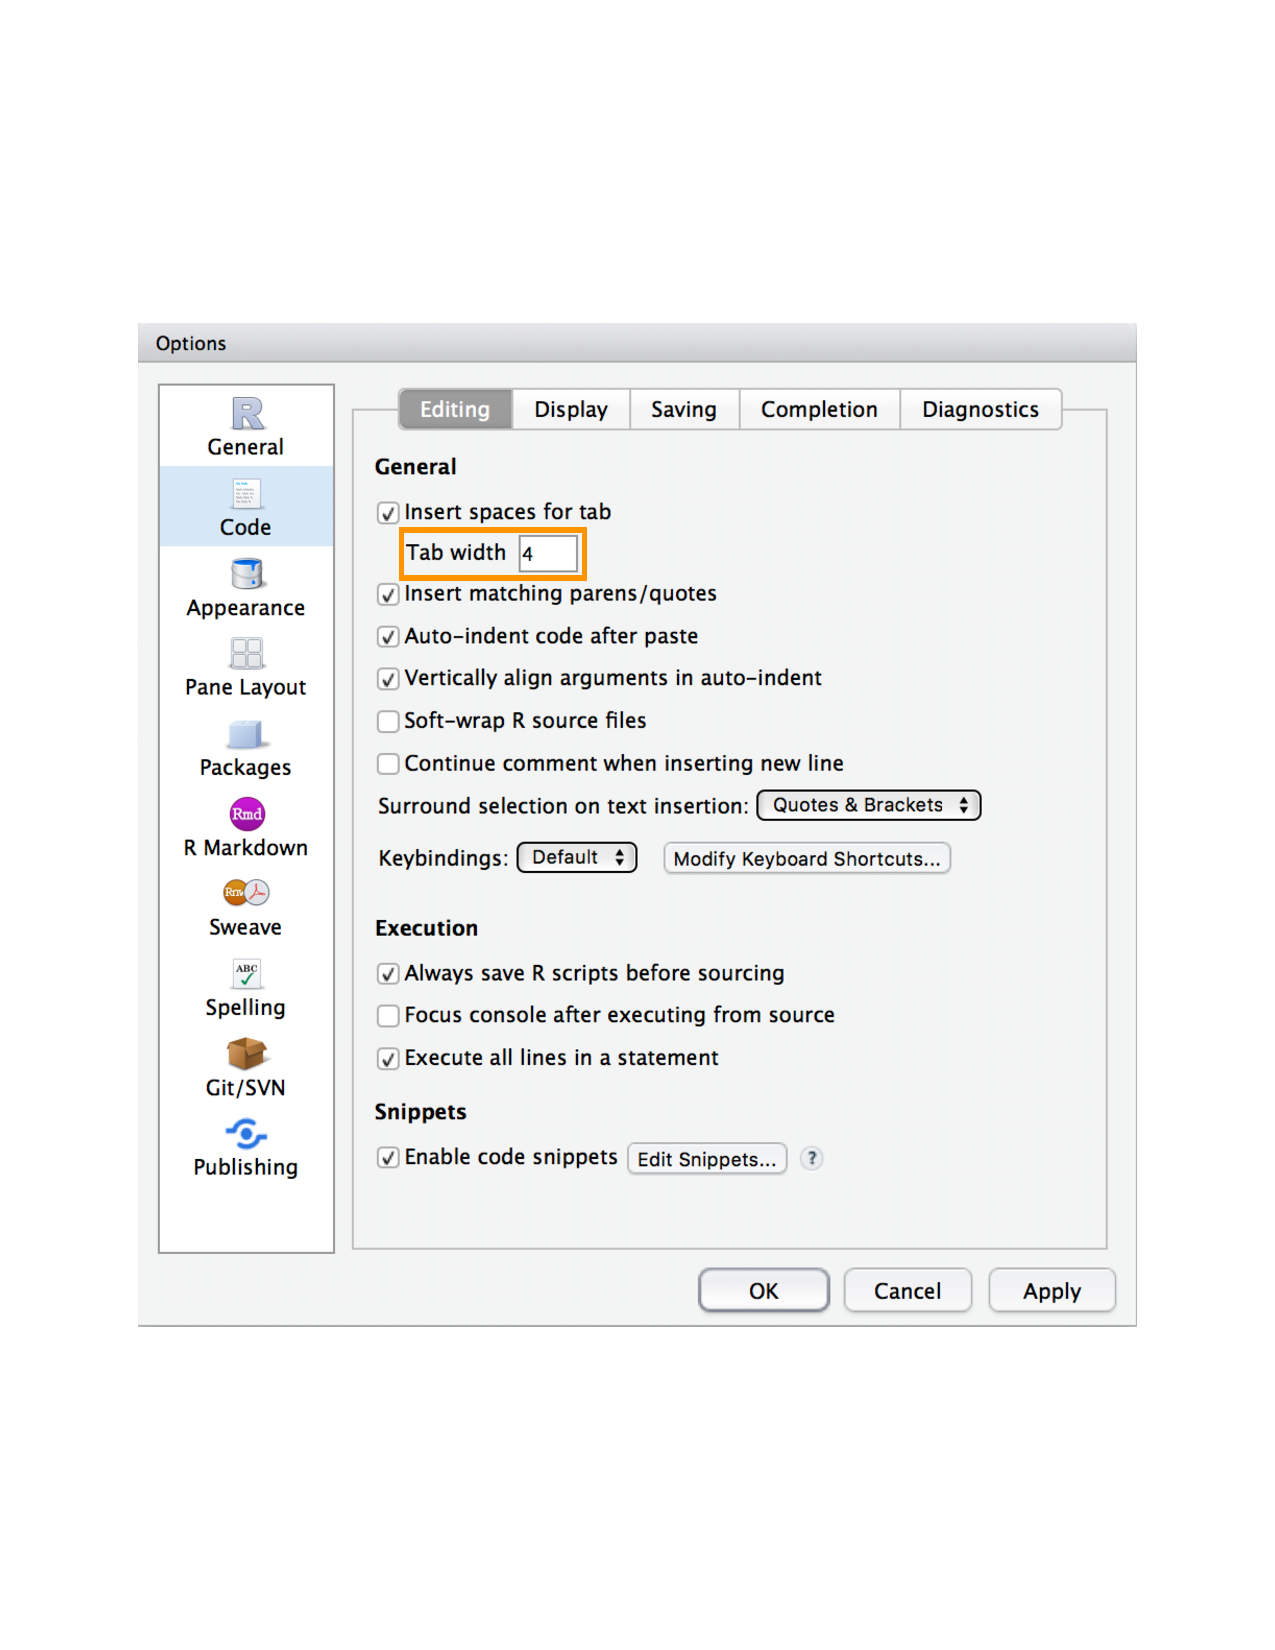
\includegraphics{rstudio-tab-width}
    \caption{Configuration de RStudio pour indenter le code de quatre
      caractères}
    \label{fig:collaboration:rstudio-tab-width}
  \end{figure}
\end{exercice}

\begin{exercice}
  Présenter le code ci-dessous selon les normes d'espacement,
  d'indentation et de positionnement des accolades mentionnées à la
  \autoref{sec:collaboration:presentation}. Pour ajuster
  automatiquement l'indentation avec RStudio, sélectionner le bloc de
  code et choisir dans les menus \code{Code|Reformat Code}.

\begin{Schunk}
\begin{Verbatim}
f <- function(x){
  if(all(x>=0)|| all(x<=0))
  { stop("all x are the same sign")
  }
  if (sum(diff(sign(x[x!=0]))!=0)>1)
  warning("more than one sign change")
 r<-polyroot(x)
i<-1/Re(r)[abs(Im(r))< .Machine$double.eps^0.5]-1
i[i > -1]
}
\end{Verbatim}
\end{Schunk}
\begin{sol}
  La présentation correcte comporte des espaces autour de tous les
  opérateurs, une indentation de quatre (4) caractères et des
  accolades ouvrante et fermante placées sur leur propre ligne.
\begin{Schunk}
\begin{Verbatim}
tri <- function(x)
{
    if (all(x >= 0) || all(x <= 0))
    {
        stop("all x are the same sign")
    }
    if (sum(diff(sign(x[x != 0])) != 0) > 1)
        warning("more than one sign change")
    r <- polyroot(x)
    i <- 1/Re(r)[abs(Im(r)) < .Machine$double.eps^0.5] - 1
    i[i > -1]
}
\end{Verbatim}
\end{Schunk}
\end{sol}
\end{exercice}

\begin{exercice}[nosol]
  Suivre le tutoriel interactif \link{https://try.github.io/}{tryGit}
  pour vous familiariser avec les commandes principales de Git.
\end{exercice}

\begin{exercice}
  Créer un compte chez \link{https://github.com}{GitHub}, puis créer
  un «embranchement» (\emph{fork}) du projet test
  \link{https://github.com/octocat/Spoon-Knife}{Spoon-Knife} depuis
  l'interface graphique de GitHub. Vous disposerez alors d'une copie
  de ce projet dans vos propres projets. Effectuer ensuite les
  opérations suivantes.
  \begin{enumerate}
  \item Cloner le projet sur votre poste de travail.
  \item Créer une branche locale pour effectuer une modification au
    projet.
  \item Modifier le fichier \code{index.html} d'une manière
    quelconque.
  \item Publier localement la modification dans la branche.
  \item Publier la branche dans le dépôt GitHub.
  \item Effectuer une «demande de tirage» (\emph{pull request}) dans
    le projet original à partir de l'interface de GitHub. Comme il
    s'agit d'un dépôt test, elle sera ignorée.
  \end{enumerate}

  \begin{sol}
    Pour créer l'embranchement (\emph{fork}), il suffit d'appuyer sur
    le bouton \code{Fork} en haut à droite de la page
    \link{https://github.com/octocat/Spoon-Knife}{Spoon-Knife}.
    Ensuite, les commandes à exécuter depuis une ligne de commande Git
    Bash (Windows) ou Terminal (macOS) sont les suivantes, dans
    l'ordre:
\begin{Schunk}
\begin{Verbatim}[commandchars=\\\{\}]
git clone https://github.com/\meta{username}/Spoon-Knife.git
cd Spoon-Knife
git checkout -b \meta{nom_branche}
\meta{modifier le fichier index.html avec son éditeur}
git status
git add index.html
git commit -m "\meta{message}"
git push -u origin \meta{nom_branche}
\end{Verbatim}
\end{Schunk}
    Enfin, retourner sur la page du projet d'origine et appuyer sur le
    bouton \code{Compare \& pull request} et suivre les instructions.
    Votre demande de tirage devrait ensuite apparaitre dans la liste
    de toutes les demandes du projet (plus de \nombre{5000} au moment
    d'écrire ces lignes).
  \end{sol}
\end{exercice}

\Closesolutionfile{solutions}


%%% Local Variables:
%%% mode: latex
%%% TeX-engine: xetex
%%% TeX-master: "programmer-avec-r"
%%% coding: utf-8
%%% End:
